\documentclass{article} % Класс печатного документа

% для поддержки русского языка
\usepackage[T2A]{fontenc} % поддержка специальных русских символов
\usepackage[utf8]{inputenc} % Кодировка исходного текста - utf8
\usepackage[english,russian]{babel} % Поддержка языка - русского с английским
\usepackage{indentfirst} % Отступ в первом абзаце

\usepackage{hyperref} % Для вставки гиперссылок
% \usepackage{listings} % Для вставки кусков кода
\usepackage{graphicx} % Вставка изображений
\usepackage{subfig} % Изображения друг напротив друга
\usepackage{float} % Для точного позиционирования картинок
\usepackage[justification=centering]{caption} % Для центрирования подписей

% Default fixed font does not support bold face
\DeclareFixedFont{\ttb}{T1}{txtt}{bx}{n}{12} % for bold
\DeclareFixedFont{\ttm}{T1}{txtt}{m}{n}{12}  % for normal

% Custom colors
\usepackage{color}
\definecolor{deepblue}{rgb}{0,0,0.5}
\definecolor{deepred}{rgb}{0.6,0,0}
\definecolor{deepgreen}{rgb}{0,0.5,0}

\usepackage{listings}

% Python style for highlighting
\newcommand\pythonstyle{\lstset{
    language=Python,
    basicstyle=\ttm,
    otherkeywords={self},             % Add keywords here
    keywordstyle=\color{deepblue},
    emph={MyClass,__init__},          % Custom highlighting
    emphstyle=\color{deepred},    % Custom highlighting style
    stringstyle=\color{deepgreen},
    frame=tb,                         % Any extra options here
    showstringspaces=false,           % 
    basicstyle=\small,                % уменьшить размер шрифта
    columns=flexible                  % чтобы при копировании не было пробелов везде
}}


% Python environment
\lstnewenvironment{python}[1][]
{
\pythonstyle
\lstset{#1}
}
{}

% Python for external files
\newcommand\pythonexternal[2][]{{
\pythonstyle
\lstinputlisting[#1]{#2}}}

% Python for inline
\newcommand\pythoninline[1]{{\pythonstyle\lstinline!#1!}}

\makeatletter
\def\lst@outputspace{{\ifx\lst@bkgcolor\empty\color{white}\else\lst@bkgcolor\fi\lst@visiblespace}}
\makeatother
 % для красивого оформления python кода

% путь к папке с изображениями
\graphicspath{{./figs/}}

\title{Отчёт 12\\
Метод опорных векторов (SVM)} % заголовок документа
\author{Свичкарев А.\,В.} % Автор документа
\date{\today} % Текущая дата

\begin{document} % Конец преамбулы, начало текста

\maketitle % Печатает заголовок, список авторов и дату

\section{Цель}
Изучить способы решения задач классификации методом опорных
векторов (SVM).

\section{Задание №1}
Написать программу построения модели классификации данных методом опорных
векторов с использованием кода из Приложения 1.
В качестве входных данных использовать случайным образом сгенерированные наборы,
представленные матрицами 20*20 и 100*100 элементов.
Применить различные типы ядер (линейный, RBF).
Визуализировать исходный набор данных и результаты классификации.
Оценить точность предсказания, затраченное время
и охарактеризовать полученные результаты.

Реализация на основе кода программы из Приложения.
\pythonexternal{../exercise1.py}

\clearpage
Визуализация исходного набора данных и результатов классификации:
\begin{figure}[H]
	\centering
	\subfloat[Обучающая выборка]{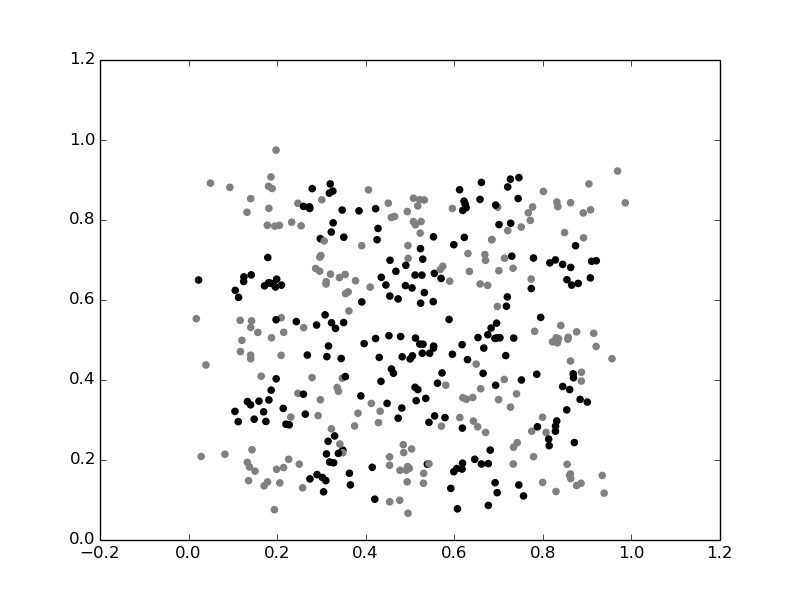
\includegraphics[width=0.5\textwidth]{ex1-train-16-kernelGauss.png}}
	\hfill
	\subfloat[Границы классов по опорным векторам]{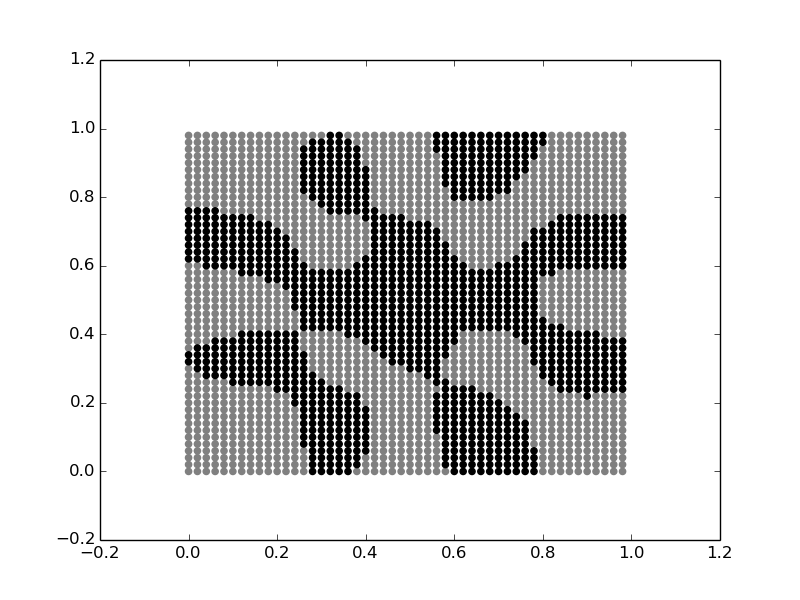
\includegraphics[width=0.5\textwidth]{ex1-class-16-kernelGauss.png}}
    \caption{Обучающая выборка 400, Гауссово ядро}
\end{figure}
\begin{figure}[H]
	\centering
	\subfloat[Обучающая выборка]{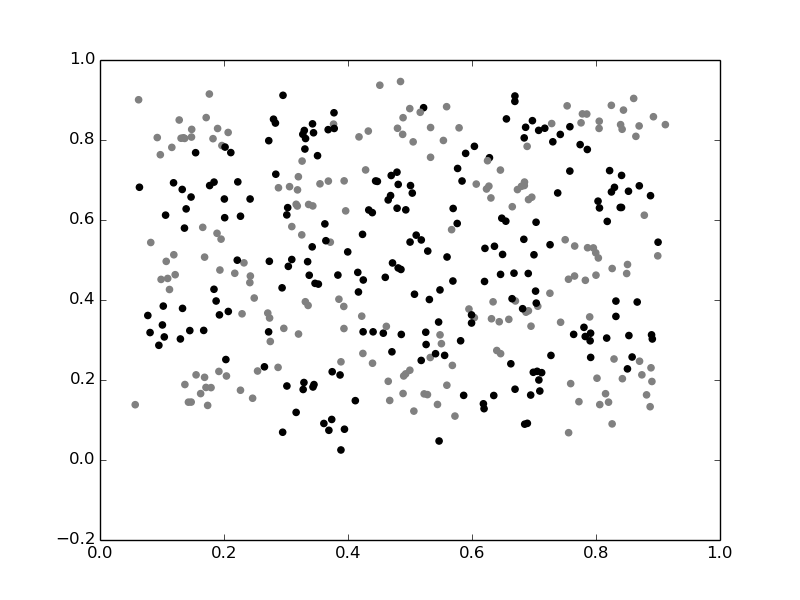
\includegraphics[width=0.5\textwidth]{ex1-train-16-kernelLinear.png}}
	\hfill
	\subfloat[Границы классов по опорным векторам]{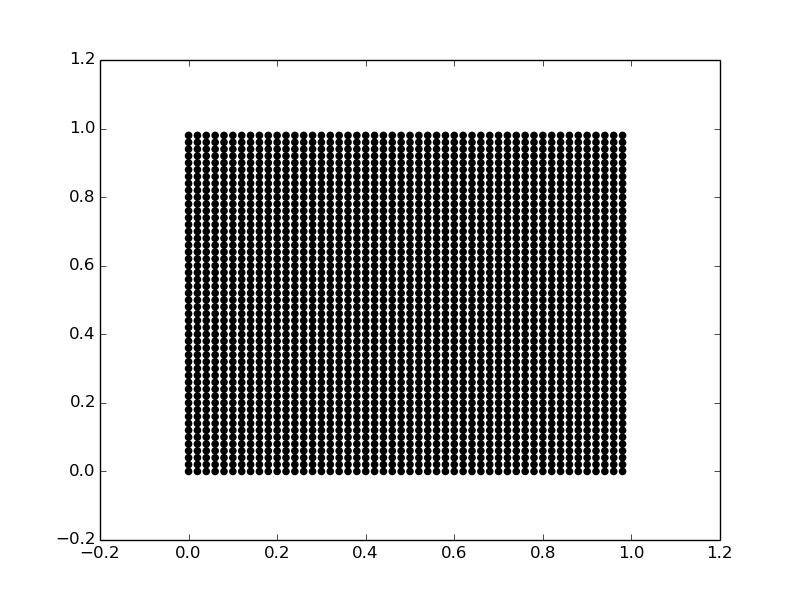
\includegraphics[width=0.5\textwidth]{ex1-class-16-kernelLinear.png}}
    \caption{Обучающая выборка 400, Линейное ядро}
\end{figure}

\begin{figure}[H]
	\centering
	\subfloat[Обучающая выборка]{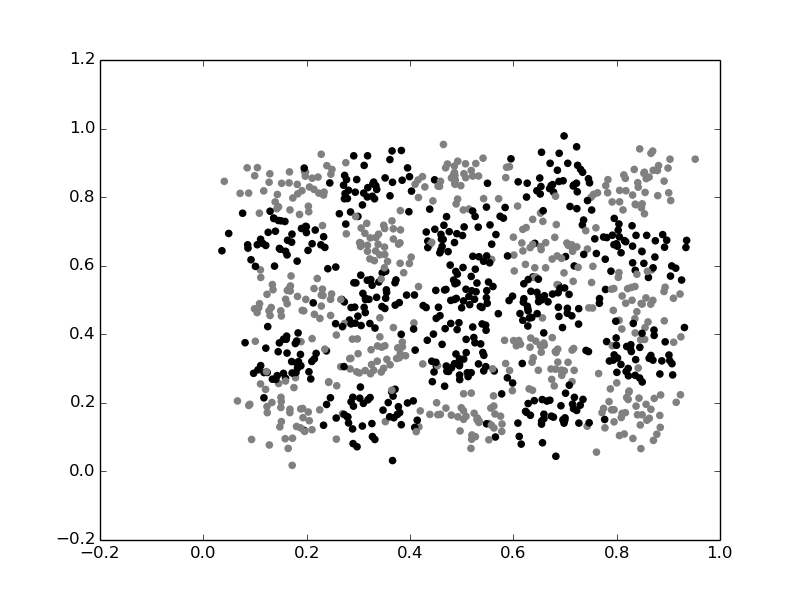
\includegraphics[width=0.5\textwidth]{ex1-train-40-kernelGauss.png}}
	\hfill
	\subfloat[Границы классов по опорным векторам]{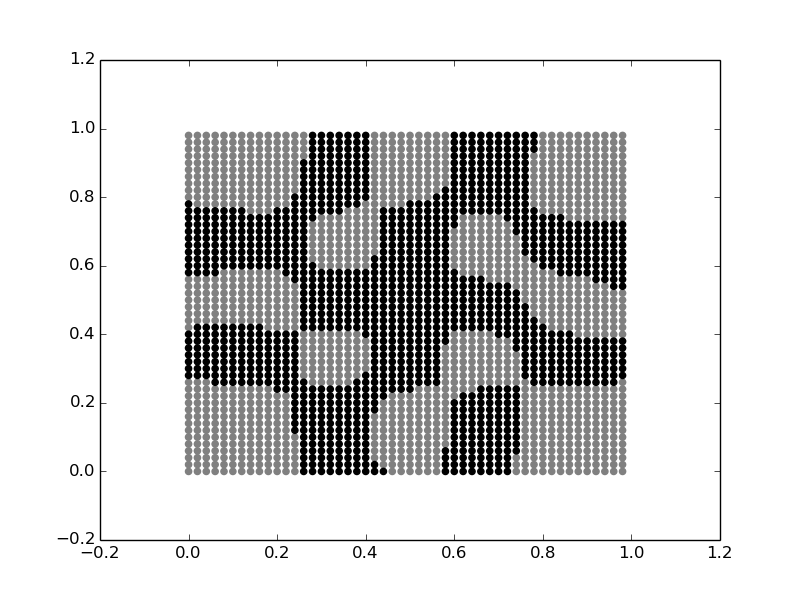
\includegraphics[width=0.5\textwidth]{ex1-class-40-kernelGauss.png}}
    \caption{Обучающая выборка 1000, Гауссово ядро}
\end{figure}
\begin{figure}[H]
	\centering
	\subfloat[Обучающая выборка]{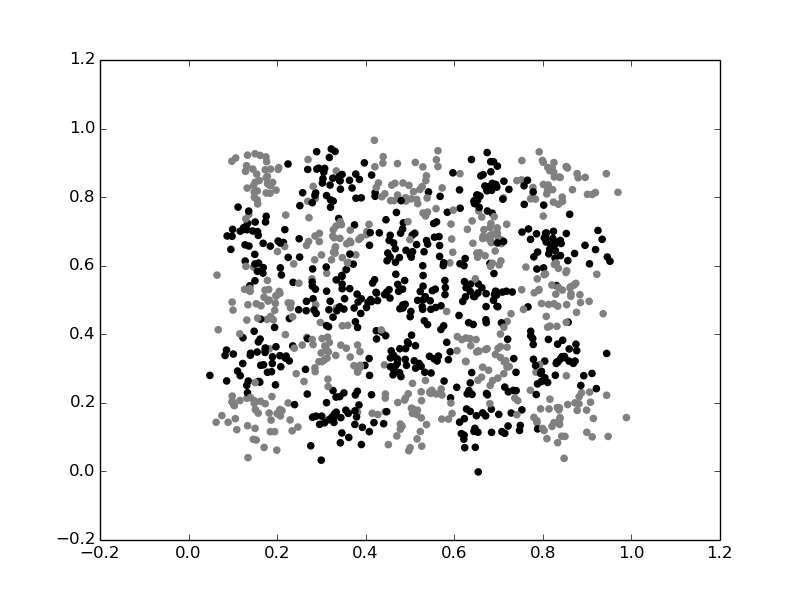
\includegraphics[width=0.5\textwidth]{ex1-train-40-kernelLinear.png}}
	\hfill
	\subfloat[Границы классов по опорным векторам]{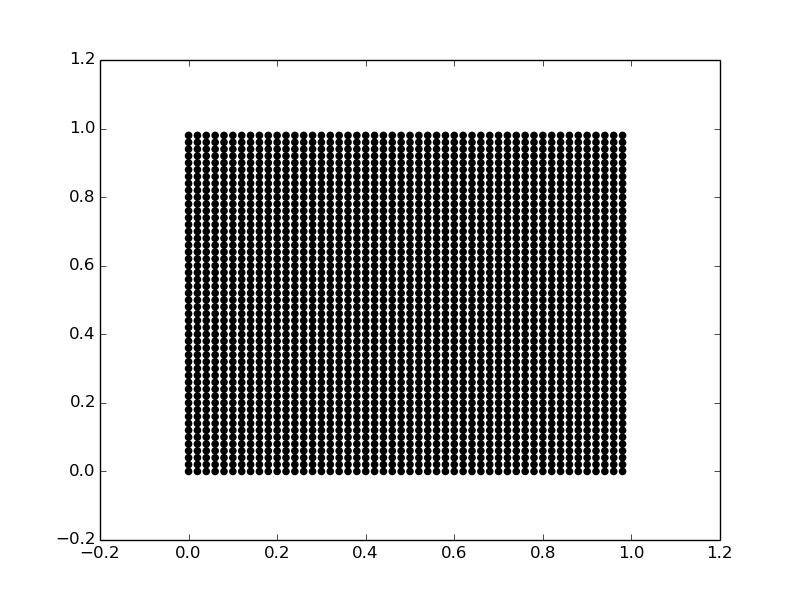
\includegraphics[width=0.5\textwidth]{ex1-class-40-kernelLinear.png}}
    \caption{Обучающая выборка 1000, Линейное ядро}
\end{figure}
\bigskip

Показатели времени и точности для результатов приведённых выше:
\lstinputlisting{ex1_out.txt}
\bigskip

\section{Задание №2}
Написать программу классификации с использованием метода svm из библиотеки
sklearn (см. Приложения 2 и 3). Применить программу к данным из первого задания.
Оценить точность, время и охарактеризовать полученные результаты в сравнении с
результатами из 1-го задания.

Реализация на основе кода программы из Приложения.
\pythonexternal{../exercise2.py}

\clearpage
Визуализация исходного набора данных и результатов классификации:
\begin{figure}[H]
	\centering
	\subfloat[Обучающая выборка]{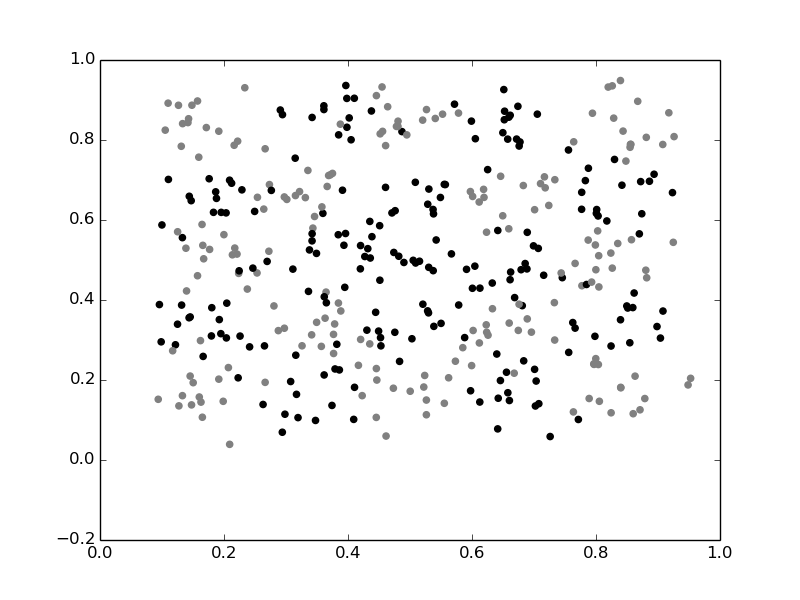
\includegraphics[width=0.5\textwidth]{ex2-train-16-kernelGauss.png}}
	\hfill
	\subfloat[Границы классов по опорным векторам]{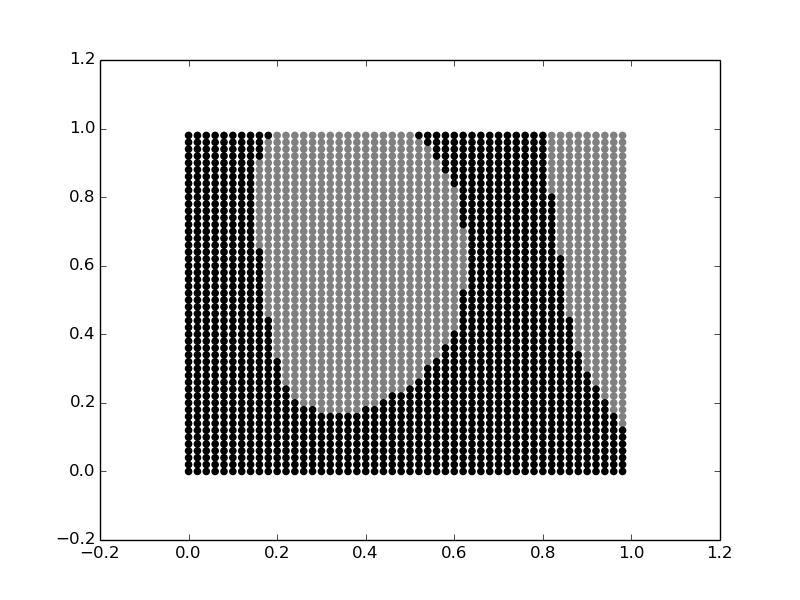
\includegraphics[width=0.5\textwidth]{ex2-class-16-kernelGauss.png}}
    \caption{Обучающая выборка 400, Гауссово ядро}
\end{figure}
\begin{figure}[H]
	\centering
	\subfloat[Обучающая выборка]{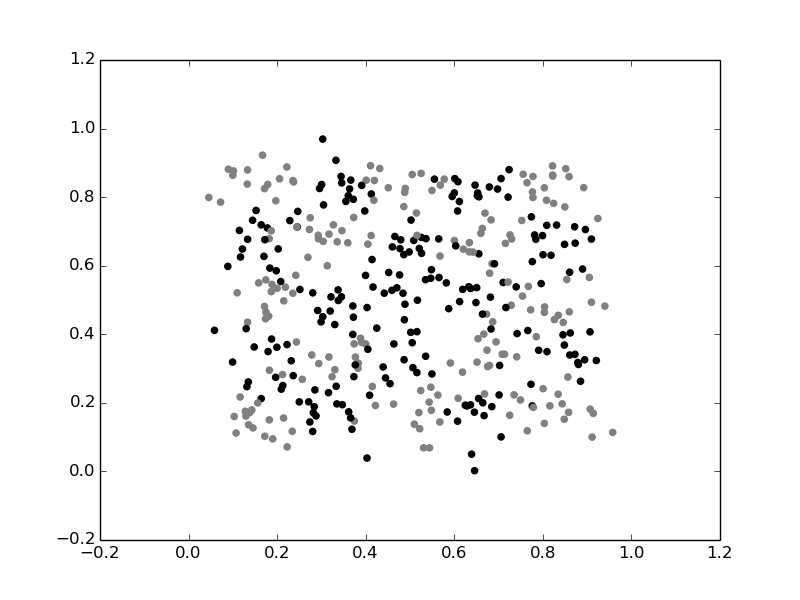
\includegraphics[width=0.5\textwidth]{ex2-train-16-kernelLinear.png}}
	\hfill
	\subfloat[Границы классов по опорным векторам]{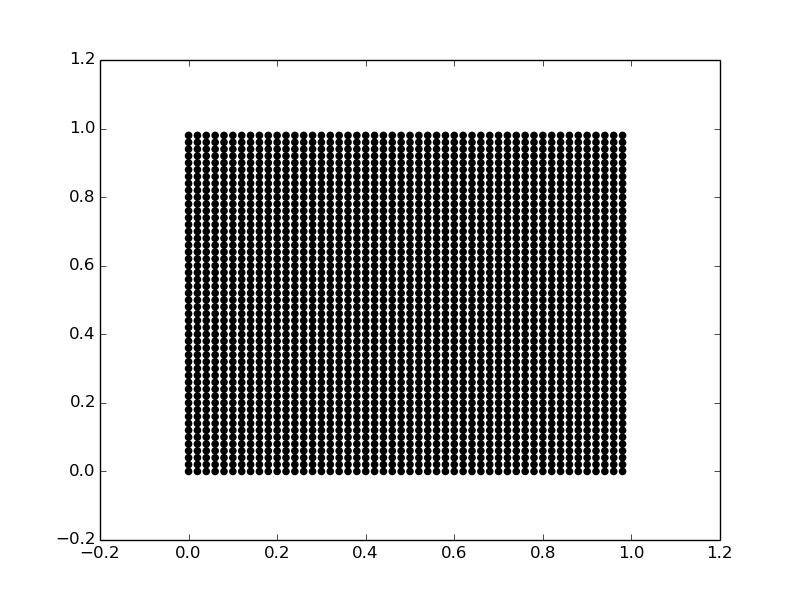
\includegraphics[width=0.5\textwidth]{ex2-class-16-kernelLinear.png}}
    \caption{Обучающая выборка 400, Линейное ядро}
\end{figure}

\begin{figure}[H]
	\centering
	\subfloat[Обучающая выборка]{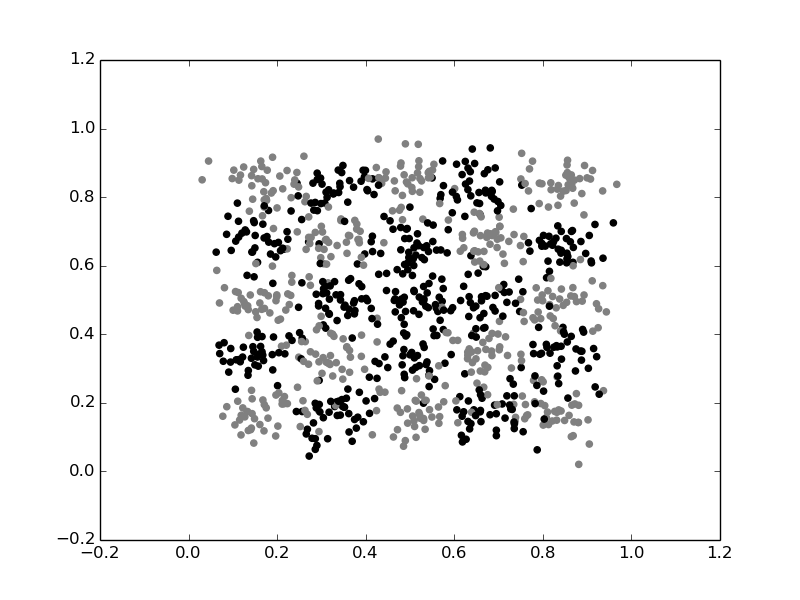
\includegraphics[width=0.5\textwidth]{ex2-train-40-kernelGauss.png}}
	\hfill
	\subfloat[Границы классов по опорным векторам]{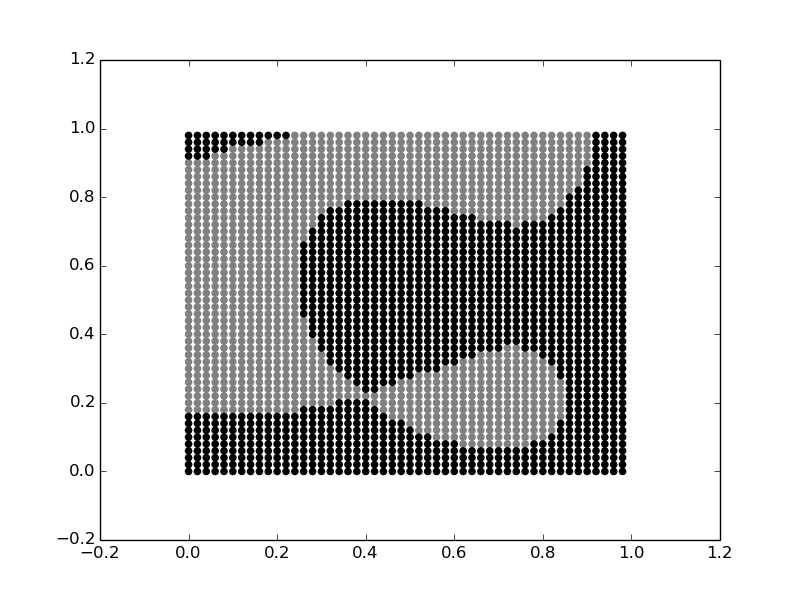
\includegraphics[width=0.5\textwidth]{ex2-class-40-kernelGauss.png}}
    \caption{Обучающая выборка 1000, Гауссово ядро}
\end{figure}
\begin{figure}[H]
	\centering
	\subfloat[Обучающая выборка]{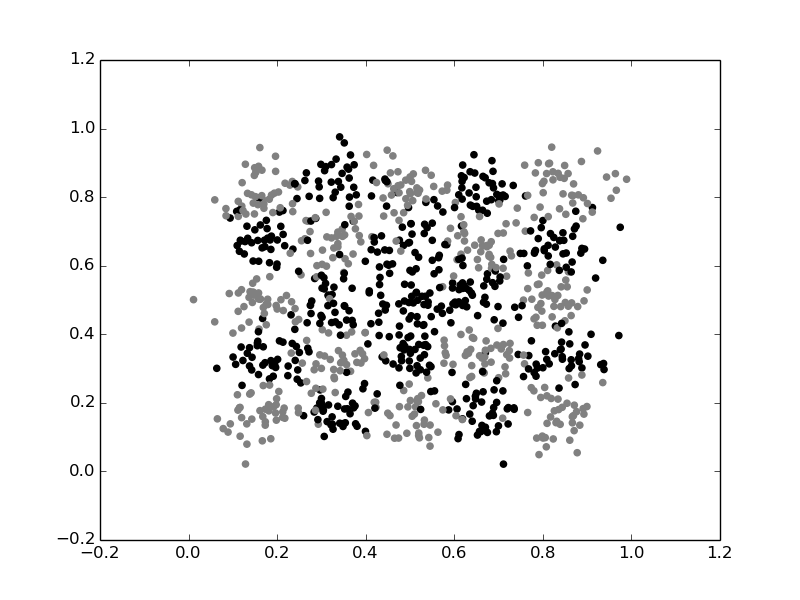
\includegraphics[width=0.5\textwidth]{ex2-train-40-kernelLinear.png}}
	\hfill
	\subfloat[Границы классов по опорным векторам]{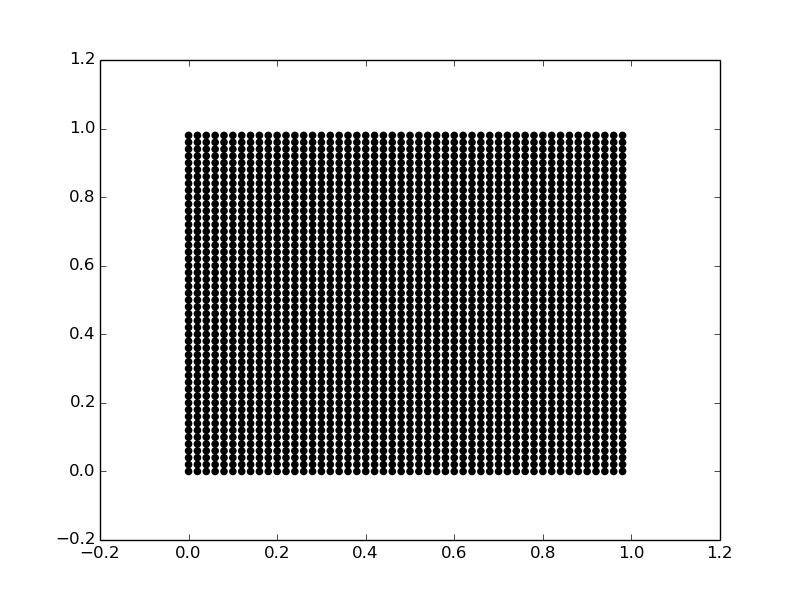
\includegraphics[width=0.5\textwidth]{ex2-class-40-kernelLinear.png}}
    \caption{Обучающая выборка 1000, Линейное ядро}
\end{figure}
\bigskip

Показатели времени и точности для результатов приведённых выше:
\lstinputlisting{ex2_out.txt}

\section{Выводы}
Для данной нелинейно разделимой выборки
линейное ядро не способно найти границу,
поэтому результат 50\%.

Гауссово ядро получает хорошие результаты (88\%)
для данного нелинейно разделимого случая,
если правильно подобраны параметры.

Задача подбора правильных параметров
является отдельной сложной задачей.

Библиотека sklearn с параметрами по умолчанию
показывает плохие результаты для гауссова ядра.
Работает на 4 порядка быстрее,
нежели самописная реализация на языке Python.

\section{Пояснение}
Исходный код доступен по ссылке:
\href{https://github.com/SvichkarevAnatoly/Course-Python-Bioinformatics/tree/master/semester2/task12}
{github.com}

\end{document} % Конец документа
